\subsection{Social Network}\label{sec:fa_social_network}

As a social platform, \emph{escolinhas.pt} makes heavy use of the social network created by its users. Due to the nature of the application, which closely mimics the Portuguese primary school system, there is a need to control how the users (especially the students and parents) interact with each other; in other words, the application needs to have mechanisms that allow the manipulation of the social network. This section describes the study and work involved in creating such mechanisms, as well as implementation details and its impact details, both in terms of variability and performance.

\subsubsection{Variability Requirements}\label{sec:fa_social_network_variability_requirements}

The current design for the escolinhas.pt social network is based on the relationships formed through the connections between users and their schools, groups, and other users, as depicted in Fig.~\ref{fig:social_network_current}. The User's Roles play an important part in the definition of this network, as an user is only linked directly to other users; any other connection is mediated through their Roles, creating their association with Schools and Groups. This allows the construction of a network where all the connections can be inferred dynamically and where an user can be identified to another through these same connections: friends, classmates, parent--child, teacher--student, and so on. This network is used mainly in the internal messaging system (and, in a brief future, the instant messaging, or chat system) of \emph{escolinhas.pt}, which allows users to communicate with each other within the platform.

\begin{figure}[H]
  \centering
  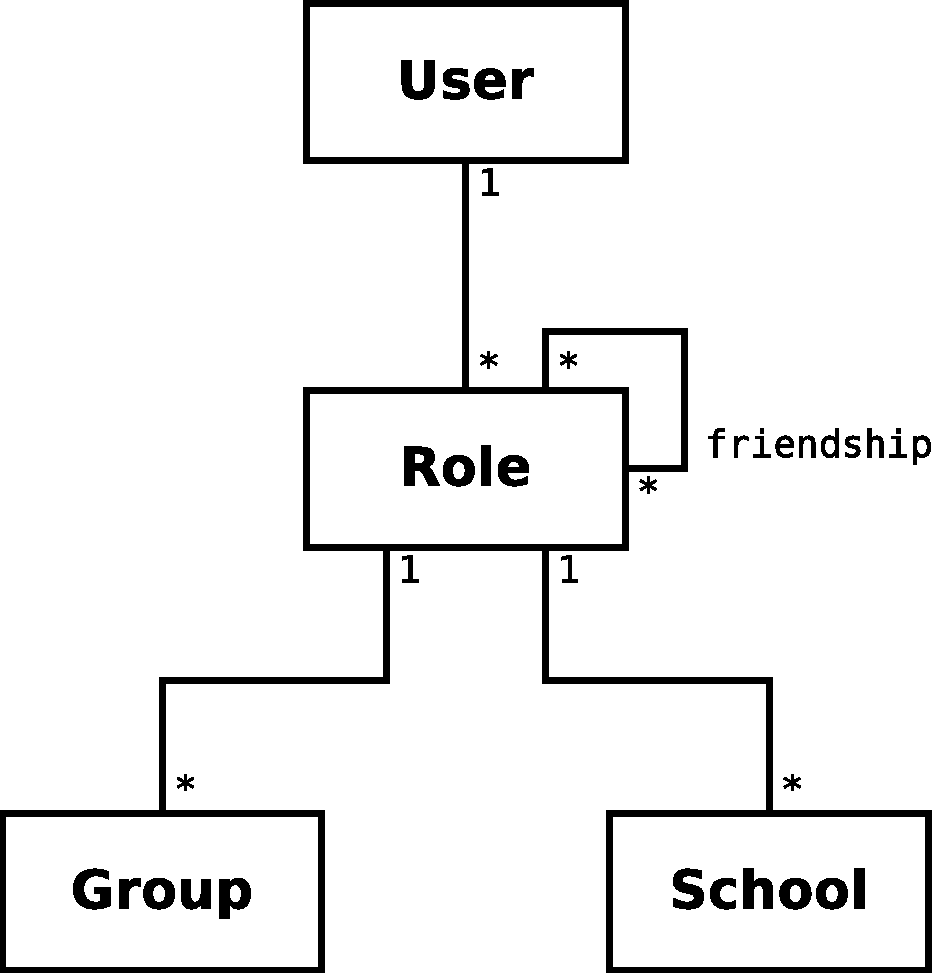
\includegraphics[width=65mm]{social_network_current.pdf}
  \caption{Current User Network Model.}
  \label{fig:social_network_current}
\end{figure}

This model, however useful, offers a very small degree of variability. Due to the closed nature of the platform, there is a need to provide mechanisms able to fine-tune these connections in order to accommodate to each school specific needs --- some Schools may not want to appear in search results; there may be some Students or even Parents who need to have special communication privileges. These mechanisms need to be available at the system administrator level, in order to easily manipulate these links without the need to pollute the application's codebase with hard-coded rules and without the need for redeployement.

\subsubsection{Candidate Patterns}\label{sec:fa_social_network_candidate_patterns}

Ideally, the user network would be described with a simple, self-referencing model, as shown in figure~\ref{fig:ideal_social_network_users}. This would allow the creation of static relationships between any two users that could be edited as needed. This would work great if all that was needed was to create relationships between users. However, it is often necessary to create connections between users and other entities in the system, such as groups and schools. Thus, this simple model needs to be abstracted in order to connect any two entities present in the system, whichever they may be, as shown in Fig.~\ref{fig:ideal_social_network_things}.

\begin{figure}[H]
  \centering
  \subfloat[Users Network]{\label{fig:ideal_social_network_users}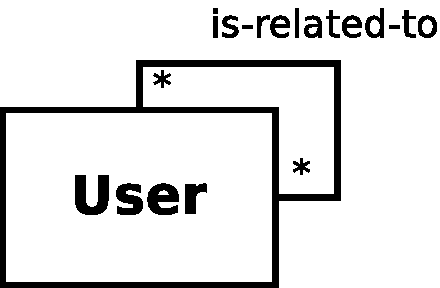
\includegraphics[width=35mm]{ideal_social_network_users}}
  \hspace{20mm}
  \subfloat[Entities Network]{\label{fig:ideal_social_network_things}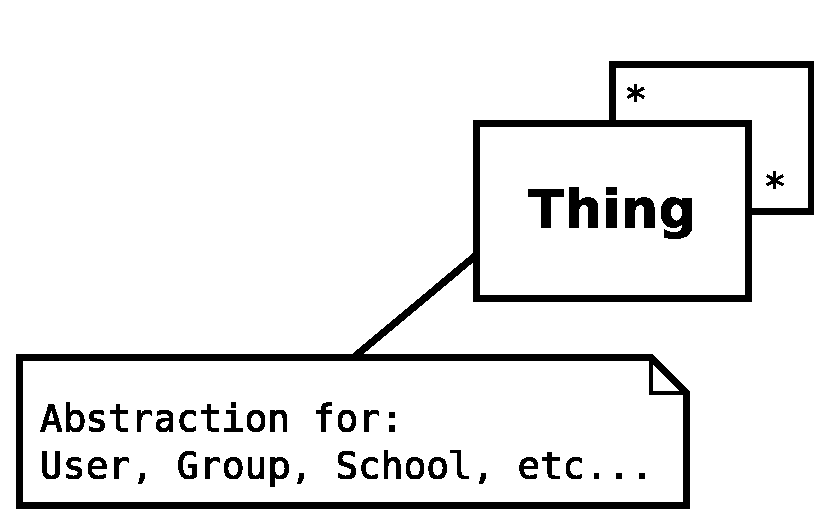
\includegraphics[width=65mm]{ideal_social_network_things}}
  \caption{Simplified Network Models.}
  \label{fig:simplified_network_models}
\end{figure}

\subsubsection{Chosen Patterns \& Rationale}\label{sec:fa_social_network_chosen_patterns_rationale}

The presented solutions are inspired by Martin Fowler's work regarding Organization Structures, and based on the \textsc{Organization Hierarchy} design pattern. Despite solving the majority of the problem, the solutions described in \ref{sec:fa_social_network_candidate_patterns} are less than ideal, as they do not allow the identification of an user towards another, because only a direct connection between two different entities is contemplated.

This could be solved by introducing an associative class containing these informations --- however, the resulting structure would still not convey enough information to properly represent the existing hierarchies, as a simple relationship between two entities (as shown in Fig.~\ref{fig:simplified_network_models}) cannot identify who is the superior and the subordinate of the relationship.

As such, for this particular problem, it is necessary to be able to connect any two entities in the system, identify their place in the hierarchy (parent or child), with an optional third entity to serve as hint as to how the original entities are connected. This problem can be solved by using the \textsc{Accountability} pattern (see \ref{sec:relationships_between_entities}) by Martin Fowler~\cite{fowler_accountability}: it allows a bi-directional, hierarchical relationship between two entities (also known as \emph{parties}) while maintaining an AccountabilityType which can be used to store additional data about the connection. As such, this AccountabilityType can be used to store an optional third party, responsible for identifying how the two other parties are connected --- effectively granting means to identify an user before an other, which is part of the original problem formulation (\ref{sec:fa_social_network}).

\subsubsection{Implementation}\label{sec:fa_social_network_implementation}

A variant of the \textsc{Accountability} design pattern (as described in section \ref{sec:relationships_between_entities}) was chosen (shown in Fig.~\ref{fig:social_network_conceptual}). This implementation follows the original description of the pattern by using all the usual entities present in the original \textsc{Accountability} pattern~\cite{fowler_accountability} --- however, it denormalizes the AccountabilityType entity \emph{into} the Accountabilities themselves, by placing the AccountabilityType attributes (\verb!type!, \verb!through!, \verb!school_year!, \verb!active!) in the Accountability. Despite creating some data redundancy, this option provides a more performant implementation: as the Accountabilities table is to be constantly accessed, the decision to have the AccountabilityTypes in a separate table would lead to expensive \verb!JOIN! operations. This, in turn, would lead to a less than desirable performance and complexity.

\begin{figure}[H]
  \centering
  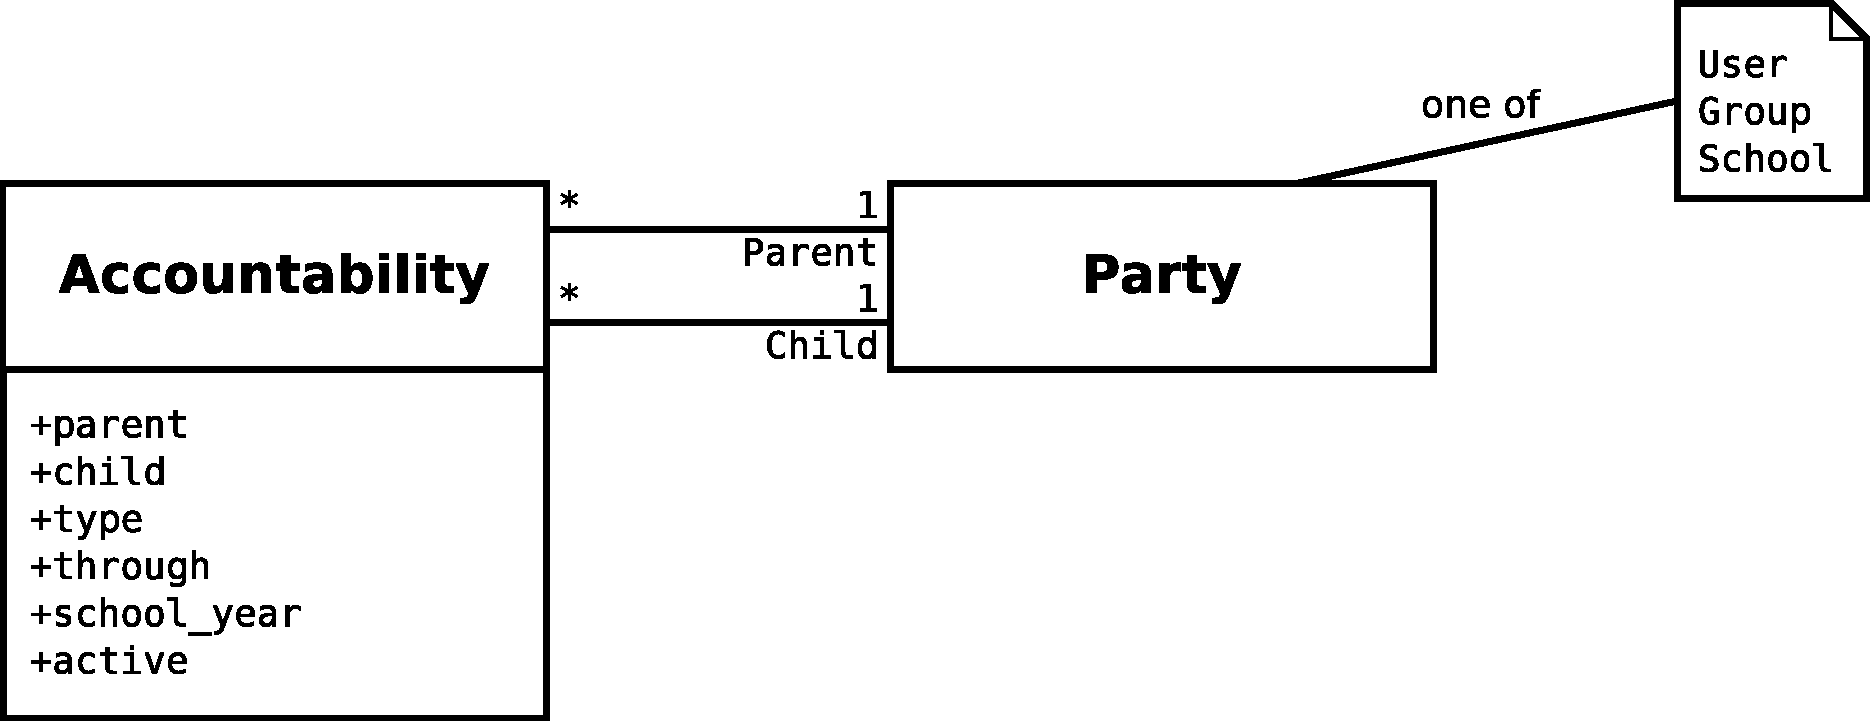
\includegraphics[width=115mm]{social_network_conceptual}
  \caption{Accountability Implementation for User Network.}
  \label{fig:social_network_conceptual}
\end{figure}

For performance reasons (explained in \ref{sec:fa_social_network_impact_analysis}), a series of different AccountabilityTypes were created, in order to cater to a multitude of relationship types, as described in Table~\ref{table:accountability_types}

%\begin{itemize}
%  \item \textbf{group\_professor:} establishes a connection between a \emph{Group} and a \emph{Professor}, meaning that the user is one of the teacher of \emph{Group}
%  \item \textbf{professor:} establishes a connection between two \emph{Users} --- a \emph{Professor} and a \emph{Student} --- creating a teacher-student relationship between them through whichever \emph{Group} they are related to
%  \item \textbf{group\_student:} establishes a connection between a \emph{Group} and a \emph{Student}, meaning that the user is part of the \emph{Group} and taught by the \textbf{group\_professors} associated with the aforementioned \emph{Group}
%  \item \textbf{school\_professor:} establishes a connection between a \emph{School} and a \emph{Professor}
%  \item \textbf{school\_student:} establishes a connection between a \emph{School} and a \emph{Student}
%  \item \textbf{parent:} establishes a parenthood relationship between two users
%  \item \textbf{school\_coordinator:} dictates an \emph{User} is a coordinator (also known as an administrator) of a certain \emph{School}
%  \item \textbf{colleague:} establishes a connection between two \emph{Users} --- either a \emph{Coordinator} or a \emph{Professor} --- through a \emph{School} they both work in
%  \item \textbf{student:} establishes a relationship between a \emph{Coordinator} and a \emph{Student} through a \emph{School}
%  \item \textbf{school\_parent:} establishes a relationship between a \emph{Coordinator} and a \emph{Parent} through a \emph{School}
%  \item \textbf{friend:} establishes a connection between any two \emph{Users} of the system --- whichever their roles may be --- to indicate a friendship relation exists between them
%\end{itemize}

% generated with http://truben.no/latex/table/

\begin{center}
  \begin{small}
    \begin{longtable}{|l|l|l|l|p{5cm}|}
      \hline
      \textbf{Type}      & \textbf{Parent} & \textbf{Child} & \textbf{Through} & \textbf{Description} \\
      \hline \hline
      group\_professor   & Group           & Professor      & ---              & establishes a connection between a \emph{Group} and a \emph{Professor}, meaning that the user is one of the teachers of \emph{Group} \\ \hline
      professor          & Professor       & Student        & Group            & establishes a connection between two \emph{Users} --- a \emph{Professor} and a \emph{Student} --- creating a teacher-student relationship between them through whichever \emph{Group} they are related to \\ \hline 
      group\_student     & Group           & Student        & ---              & establishes a connection between a \emph{Group} and a \emph{Student}, meaning that the user is part of the \emph{Group} and taught by the \textbf{group\_professors} associated with the aforementioned \emph{Group} \\ \hline 
      school\_professor  & School          & Professor      & ---              & establishes a connection between a \emph{School} and a \emph{Professor} \\ \hline 
      school\_student    & School          & Student        & ---              & establishes a connection between a \emph{School} and a \emph{Student} \\ \hline 
      parent             & Parent          & Student        & ---              & establishes a parenthood relationship between two users \\ \hline 
      school\_cordinator & School          & Coordinator    & ---              & dictates an \emph{User} is a coordinator (also known as an administrator) of a certain \emph{School} \\ \hline 
      colleague          & Professor       & Coordinator    & School           & establishes a connection between two \emph{Users} --- either a \emph{Coordinator} or a \emph{Professor} --- through a \emph{School} they both work in \\ \hline 
      student            & Coordinator     & Student        & School           & establishes a relationship between a \emph{Coordinator} and a \emph{Student} through a \emph{School} \\ \hline 
      school\_parent     & Coordinator     & Parent         & School           & establishes a relationship between a \emph{Coordinator} and a \emph{Parent} through a \emph{School} \\ \hline 
      friend             & User            & User           & ---              & establishes a connection between any two \emph{Users} of the system --- whichever their roles may be --- to indicate a friendship relation exists between them \\ \hline
    
    \caption{AccountabilityTypes created to describe every type of existent relation.}
    \label{table:accountability_types}
    \end{longtable}
  \end{small}
\end{center}

Some of the aforementioned AccountabilityTypes are representative of every type of interpersonal relationship existent in the escolinhas.pt platform. At first sight, some of the AccountabilityTypes created may seem redundant, such as student and school\_parent: they exist because the school coordinator needs to be able to contact everyone who is part of the school. One could argue these connections could easily be inferred through the relations between the coordinator and his or her school, and the relations existent between the school and its students, and finally use the existent parenthood relationships. However, as described in \ref{sec:fa_social_network_variability_requirements}, one of the major design flaws (regarding variability), was the completely dynamic nature of the contacts network --- as the network was always built upon request, there was no viable way of modifying it without using hardcoded rules or a configuration setup external to the code. Thus, the choice to implement apparently redundant AccountabilityTypes tied itself with the necessity to have full control over the existent social relationships. The remainder of the AccountabilityTypes are used to store and facilitate access to membership-like relationships, by stating a certain user is part of a school or group at a given school year. This also allows the platform to keep a history of past (inactive) relationships between entities in the system.

\subsubsection{Impact Analysis}\label{sec:fa_social_network_impact_analysis}

The usage of this design pattern not only solved some of the existing variability and performance problems, but introduced a new possibility: the ability to create relationships between any two entities in the system. This leads to a very flexible network, capable of being modified at the M0 (data) level (see \ref{sec:aom_architecture}), which is a pre-requisite for end-user level variability.

A second objective pertaining to the application of this pattern was to improve the performance related to contact list creation and the identification of these before the user. This task is currently extremely expensive, with an edge case of 5724 queries needed to fetch and identify 715 contacts. A user with only 18 contacts generates 154 queries. This means that an average of 8 queries are performed for each one of the contacts, meaning the cost of this operation is approximately linear in nature, as depicted in Fig.~\ref{fig:contact_queries}.

\begin{figure}[H]
  \centering
  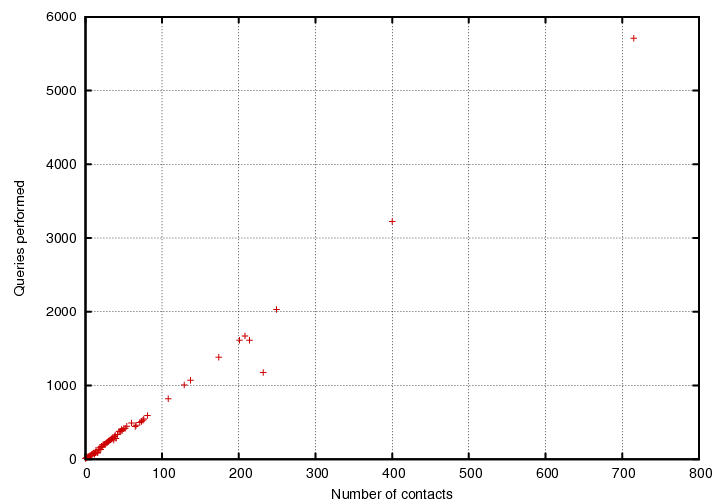
\includegraphics[width=145mm]{graphs/contact_queries}
  \caption{Average number of queries performed per number of contacts.}
  \label{fig:contact_queries}
\end{figure}

The graph in Fig.~\ref{fig:contact_queries} represents the average number of queries performed per number of contacts a user has, and it was sampled from a random population of 10000 real users of the platform. As stated before cost growth of the function is only approximately linear: due to the dynamic nature of the network, some users may have a sparser network --- e.g. less groups associated with, but more users associated with each group the user is part of --- which can explain the unexpected decrease in the number of queries around the 200-mark and the irregularities in users with less than 100 contacts. However, in practice, this cost can be extrapolated to a linear cost, to a point where one can infer that the number of queries performed is approximately 8 times the number of contacts, which represents a very serious performance issue for one of the most used features of the platform.

%The data used to build the chart can be found in \nameref{sec:appendix_a}

The implementation of the \textsc{Accountability} pattern to maintain the relationships between users was able to reduce the cost of the abovementioned task to $O(1)$: only 11 queries are performed to fetch and identify an user contacts, regardless of the size of said contact list. This means that the platform is able to sustain a considerable growth without suffering serious impacts on the performance of seemingly trivial operations.

